\section{Projections for LHC neutrino structure functions}
\label{sec:dis_pseudodata}

We begin by describing the procedure adopted to generate
projections for DIS structure functions associated to LHC neutrinos.
%
Assembling these projections requires defining the kinematic acceptance
and expected yields of the various ongoing and proposed experiments,
assessing the performance of their response in order to estimate
the corresponding systematic uncertainties,
and then evaluating pseudo-data based on specific underlying theory assumption which should be consistent
with the settings of the subsequent (nuclear) PDF analyses.

In this section, for completeness first of all we provide a recap of the kinematics
of neutrino DIS structure function measurements.
%
Then we present an overview of the LHC far-forward neutrino detectors that
will be considered in the present study.
%
The calculation of event yields in bins of $x,Q^2$, and neutrino energy $E_\nu$ in terms
of the incoming neutrino fluxes is presented next, resulting in quantitative predictions
for the kinematic coverage and statistical uncertainties.
%
Finally, we discuss how for each of the considered experiments the dominant systematic
uncertainties are evaluated and which assumptions are taken about their bin-to-bin correlations.


\subsection{Neutrino deep-inelastic scattering}

The theoretical framework underlying neutrino DIS is well known, see e.g.~\cite{Candido:2023utz}
and references therein.
%
For completeness, we provide here a short overview of the neutrino DIS formalism.
%
The double-differential cross-section for neutrino-nucleus charged-current scattering
can be expressed in terms of three
independent structure functions $F_2^{\nu A}(x,Q^2)$, $xF_3^{\nu A}(x,Q^2)$
and $F_L^{\nu A}(x,Q^2)$ as follows
\be
\label{eq:neutrino_DIS_xsec_FL}
\frac{d^2\sigma^{\nu A}(x,Q^2,y)}{dxdy} =  \frac{G_F^2s/4\pi}{\lp 1+Q^2/m_W^2\rp^2}\lc Y_+F^{\nu A}_2(x,Q^2) - y^2F^{\nu A}_L(x,Q^2) +Y_- xF^{\nu A}_3(x,Q^2)\rc  \, ,
\ee
where $Y_\pm = 1 \pm (1-y)^2$ and with a counterpart expression for anti-neutrino scattering,
\be
\label{eq:antineutrino_DIS_xsec_FL}
\frac{d^2\sigma^{\bar{\nu} A}(x,Q^2,y)}{dxdy} =  \frac{G_F^2s/4\pi}{\lp 1+Q^2/m_W^2\rp^2}\lc Y_+F^{\bar{\nu} A}_2(x,Q^2) - y^2F^{\bar{\nu} A}_L(x,Q^2) -Y_- xF^{\bar{\nu} A}_3(x,Q^2)\rc  \, ,
\ee
where $s=2m_N E_\nu$ is the neutrino-nucleon center of mass energy squared, $m_N$ is the nucleon mass,
$E_\nu$ is the incoming neutrino energy,
and the inelasticity is $y=Q^2/(2x m_n E_{\nu})$.
%
While structure functions depend only on $x$ and $Q^2$, the differential
cross-section depends also on the neutrino energy $E_\nu$ (or alternatively
on the inelasticity $y$).
%
Structure functions $F^{\nu A}_i(x,Q^2)$ and $F^{\bar{\nu} A}_i(x,Q^2)$ depend on the nuclear target $A$ entering
for the neutrino scattering through the nuclear modifications of the proton PDFs.

Eqns.~(\ref{eq:neutrino_DIS_xsec_FL}) and~(\ref{eq:antineutrino_DIS_xsec_FL}) are valid in the  inelastic
scattering regime, defined as the kinematic region for which the 
hadronic final-state
invariant mass $W$  satisfies
\be
W^2 = \lp m_N^2 + Q^2 \frac{(1-x)}{x} \rp \gsim \lp 2\,{\rm GeV} \rp^2\, ,
\ee
given that for smaller values of $W^2$  neutrino scattering is dominated by either quasi-elastic scattering
or the resonance production region.
%
Provided the momentum transfer becomes large enough, $Q^2 \gsim {\rm few~GeV}^2$,
the inelastic structure functions Eqns.~(\ref{eq:neutrino_DIS_xsec_FL}) and~(\ref{eq:antineutrino_DIS_xsec_FL})
can be decomposed in terms of a convolution of partonic scattering cross-sections  $C_{i,j}^{\nu N}(x,\alpha_s)$ and
of process-independent PDFs $f^{(A)}_j\lp x,Q^2\rp$, 
\be
\label{eq:sfs_pqcd}
 F^{\nu A}_i(x,Q^2) = \sum_{j=q,\bar{q},g}\int_x^1 \frac{dz}{z}\, C_{i,j}^{\nu N}(z,\alpha_s(Q^2))f^{(A)}_j\lp \frac{x}{z},Q^2\rp \, , \quad i = 2,3,L \, .
 \ee
 Eq.~(\ref{eq:sfs_pqcd}) holds both for inclusive and for heavy quark production structure functions,
 thought in the latter case one needs to account for mass-dependent effects.
 %
 Neutrino structure functions can be computed up to N$^3$LO for the massless case
 and up to NNLO (with respect to the Born cross-section) for the charm production
 case~\cite{Gao:2017kkx}.
 %
 We discuss in Sect.~\ref{sec:settings} the
 tools~\cite{Candido:2022tld,yadism,Candido:2023utz,Carrazza:2020gss} used in this work to
 evaluate neutrino DIS structure functions in order to generate
 LHC neutrino pseudo-data.
 %
 In this work we don't consider structure functions in the shallow inelastic scattering region (SIS)
 defined by $Q^2 \lsim {\rm few~GeV}^2$, for which a different approach
 must the  adopted for their evaluation~\cite{Candido:2023utz}.

 Each different structure function provides complementary sensitivity
 to the partonic flavour decompositions of nucleons.
 %
 To illustrate this sensitivity, one can consider a leading order (LO) calculation
 for a proton target, $n_f=4$ active quark flavours,
 neglecting charm mass effects and assuming a diagonal CKM matrix.
 %
 In this scenario one can express the $F_2^{\nu p}$ and $xF_3^{\nu p}$ structure functions as
 follows:
 \bea
 F_2^{\nu p}(x,Q^2) &=& 2x\lp f_{\bar{u}} + f_{d} + f_{s} + f_{\bar{c}} \rp(x,Q^2) \, , \nonumber  \\
 F_2^{\bar{\nu} p}(x,Q^2) &=& 2x\lp f_u + f_{\bar{d}} + f_{\bar{s}} + f_c \rp(x,Q^2) \, , \label{eq:neutrinoSFs} \\
 xF_3^{\nu p}(x,Q^2) &=& 2x\lp -f_{\bar{u}} + f_d +f_s - f_{\bar{c}}\rp(x,Q^2)  \, , \nonumber\\
 xF_3^{\bar{\nu} p}(x,Q^2) &=& 2x\lp f_u - f_{\bar{d}} -f_{\bar{s}} + f_{c}\rp(x,Q^2) \, . \nonumber
 \eea
 The corresponding expressions for a neutron target are obtained from isospin symmetry
 \bea
 F_2^{\nu n}(x,Q^2) &=& 2x\lp f_{\bar{d}} + f_{u} + f_{s} + f_{\bar{c}} \rp(x,Q^2) \, , \nonumber  \\
 F_2^{\bar{\nu} n}(x,Q^2) &=& 2x\lp f_d + f_{\bar{u}} + f_{\bar{s}} + f_c \rp(x,Q^2) \, , \label{eq:antineutrinoSFs} \\
 xF_3^{\nu n}(x,Q^2) &=& 2x\lp -f_{\bar{d}} + f_u +f_s - f_{\bar{c}}\rp(x,Q^2)  \, , \nonumber\\
 xF_3^{\bar{\nu} n}(x,Q^2) &=& 2x\lp f_d - f_{\bar{u}} -f_{\bar{s}} + f_{c}\rp(x,Q^2) \, , \nonumber
 \eea
 while for an isoscalar, free-nucleon target denoted by $N$ one has
 \bea
 F_2^{\nu N}(x,Q^2) &=& 2x\lp f_{u^+} + f_{d^+} + 2f_s + 2f_{\bar{c}} \rp(x,Q^2) \, , \nonumber  \\
 F_2^{\bar{\nu} N}(x,Q^2) &=& 2x\lp f_{u^+} + f_{d^+} + 2f_{\bar{s}} + 2f_c \rp(x,Q^2) \, , \label{eq:neutrinoSFs} \\
 xF_3^{\nu N}(x,Q^2) &=& 2x\lp f_{u^-} + f_{d^-} +2f_s - 2f_{\bar{c}}\rp(x,Q^2)  \, , \nonumber\\
 xF_3^{\bar{\nu} N}(x,Q^2) &=& 2x\lp   f_{u^-} + f_{d^-}-2f_{\bar{s}} +2 f_{c}\rp(x,Q^2) \, , \nonumber
 \eea
 in terms of the valence and sea PDF combinations defined by
 \be
 f_{q^+} (x,Q^2)\equiv \lp f_{q}+f_{\bar{q}}\rp(x,Q^2) \, , \qquad
 f_{q^-} (x,Q^2)\equiv \lp f_{q}- f_{\bar{q}}\rp(x,Q^2) \, .
 \ee
 From this partonic decomposition we see that even for isoscalar targets separate measurements
 for neutrinos and antineutrinos are not equivalent since in general neither $f_{s^-}$ nor
 $f_{c^-}$ are expected to vanish.

 In the projections presented in this work, when interpreting the LHC neutrino structure
 functions in terms of proton PDFs we assume isoscalar free-nucleon targets and neglect
 nuclear PDF modifications.
 %
 When evaluating structure functions for a tungsten (W) target, we keep into account
 that the target is not isoscalar when evaluating the physical observables.
 

 \subsection{Far-forward neutrino detectors at the LHC}
 \label{sec:neutrinoDetectors}
 

\subsection{DIS pseudo-data generation}
\label{sec:pseudo-data_generation}

The first goal is to produce projections
for DIS pseudo-data at the FPF based on
some idealised detector concepts and
some initial choice of neutrino fluxes
e.g.~\cite{Kling:2021gos}.
%
This requires a knowledge of the detector geometry
and material, as well as of the double-differential
neutrino interaction cross-section. 
%
Since we aim to produce pseudo-data binned in $(x,Q^2)$,
for each simulated event we need to determine the 
final-state kinematics. 

Specifically, we would like to evaluate the
number of charged-current neutrino interaction events
within the detector volume in different bins
of the incoming neutrino energy $E_\nu$, the Bjorken
variable $x$ and the momentum transfer square $Q^2$,
\begin{equation}
    N_{\rm ev}(E_\nu, x, Q^2) \, ,
\end{equation}
for some binning in these three kinematic variables.
%
This can be evaluated as
\begin{equation}
\label{eq:nev_v1}
    N_{\rm ev}(E_\nu, x, Q^2) \propto \int_{\rm bin}\int_{\rm det}  \frac{d^2\sigma^{\nu A}(x,Q^2,y)}{dxdy} \mathcal{L}_{\nu}(E_{\nu}) \, ,
\end{equation}
where $\mathcal{L}(E_{\nu}) $ is the incoming neutrino
luminosity which accounts for the detector geometry
and material density. 
%
Eq.~(\ref{eq:nev_v1}) can be integrated to
determine the actual number of events within
the bin boundaries.

We start with a perfect detector.


For bins in $x,Q^2,E_{\nu}$, we start with the \href{https://github.com/juanrojochacon/FPF-WG1/blob/main/results/diff_xsecs_a1.txt}{differential cross section},$\frac{d^2\sigma(x,Q^2,E_{\nu}}{dxdQ^2})$ [pb GeV$^{-2}$] as output from {\tt YADISM} and convolve with the \href{https://github.com/KlingFelix/FastNeutrinoFluxSimulation/tree/main/Fluxes}{neutrino flux}, $\frac{dN_{\nu}}{dE_{\nu}}$. So for a detector with $n_T$ nuclear target density and $L_T$ length, we calculate the event rate per bin as

\begin{equation}
    N_{\rm ev}/{\rm bin} = n_T L_T\int_{Q^2_{min}}^{Q^2_{max}}\int_{x_{min}}^{x_{max}}\int_{E_{\nu,min}}^{E_{\nu , max}} \frac{dN_{\nu}}{dE_{\nu}}\left(\frac{d^2\sigma(x,Q^2,E_{\nu})}{dxdQ^2}\right) dQ^2 dx dE_{\nu}.
\end{equation}

Using a MC integration, we can calculate $N_{\rm ev}/{\rm bin}$ by sampling $N$ points in $x,Q^2,E_{\nu}$ space such that $0< y = \frac{Q^2}{2m_N E_{\nu }x} < 1$ and integrating over the bin.

\begin{equation}
    N_{\rm ev}/{\rm bin} \approx n_T L_T \frac{(Q^2_{max}-Q^2_{min})(x_{max}-x_{min})(E_{\nu ,max}-E_{\nu ,min})}{N}\times \sum_i^N f(x_i,Q^2_i,E_{\nu ,i})
    \label{MCintegration}
\end{equation}

where $f(x_i,Q^2_i,E_{\nu ,i}) = \frac{dN_{\nu}}{dE_{\nu,i}}\left(\frac{d^2\sigma(x_i,Q^2_i,E_{\nu,i})}{dxdQ^2}\right)$. 

The statistical uncertainty for each bin is then defined by a Gaussian distribution with fractional uncertainty $1/\sqrt{N{\rm ev}/{\rm bin}}$, i.e. $\delta N_{\rm ev}/{\rm bin} = \sqrt{N_{\rm ev}} /{\rm bin}$


  Following this prescription, we can produce plots which characterize the event rate for a particular neutrino species at a particular experiment. 

Results for FASER$\nu$2 can be found \href{https://github.com/juanrojochacon/FPF-WG1/tree/main/results}{here}. The .txt files will display which neutrino species was considered, and also compile experimental geometries and target details in the header. In the sub-folder \href{https://github.com/juanrojochacon/FPF-WG1/tree/main/results/Summaries}{summaries}, plots can be found which show the event rate in $x,Q^2$ space, integrating over the entire neutrino spectrum. The event rate for muon neutrinos at FASER$\nu$2 is shown in Fig~\ref{fig:fasernu2_muon}.

\begin{figure}[h]
    \centering
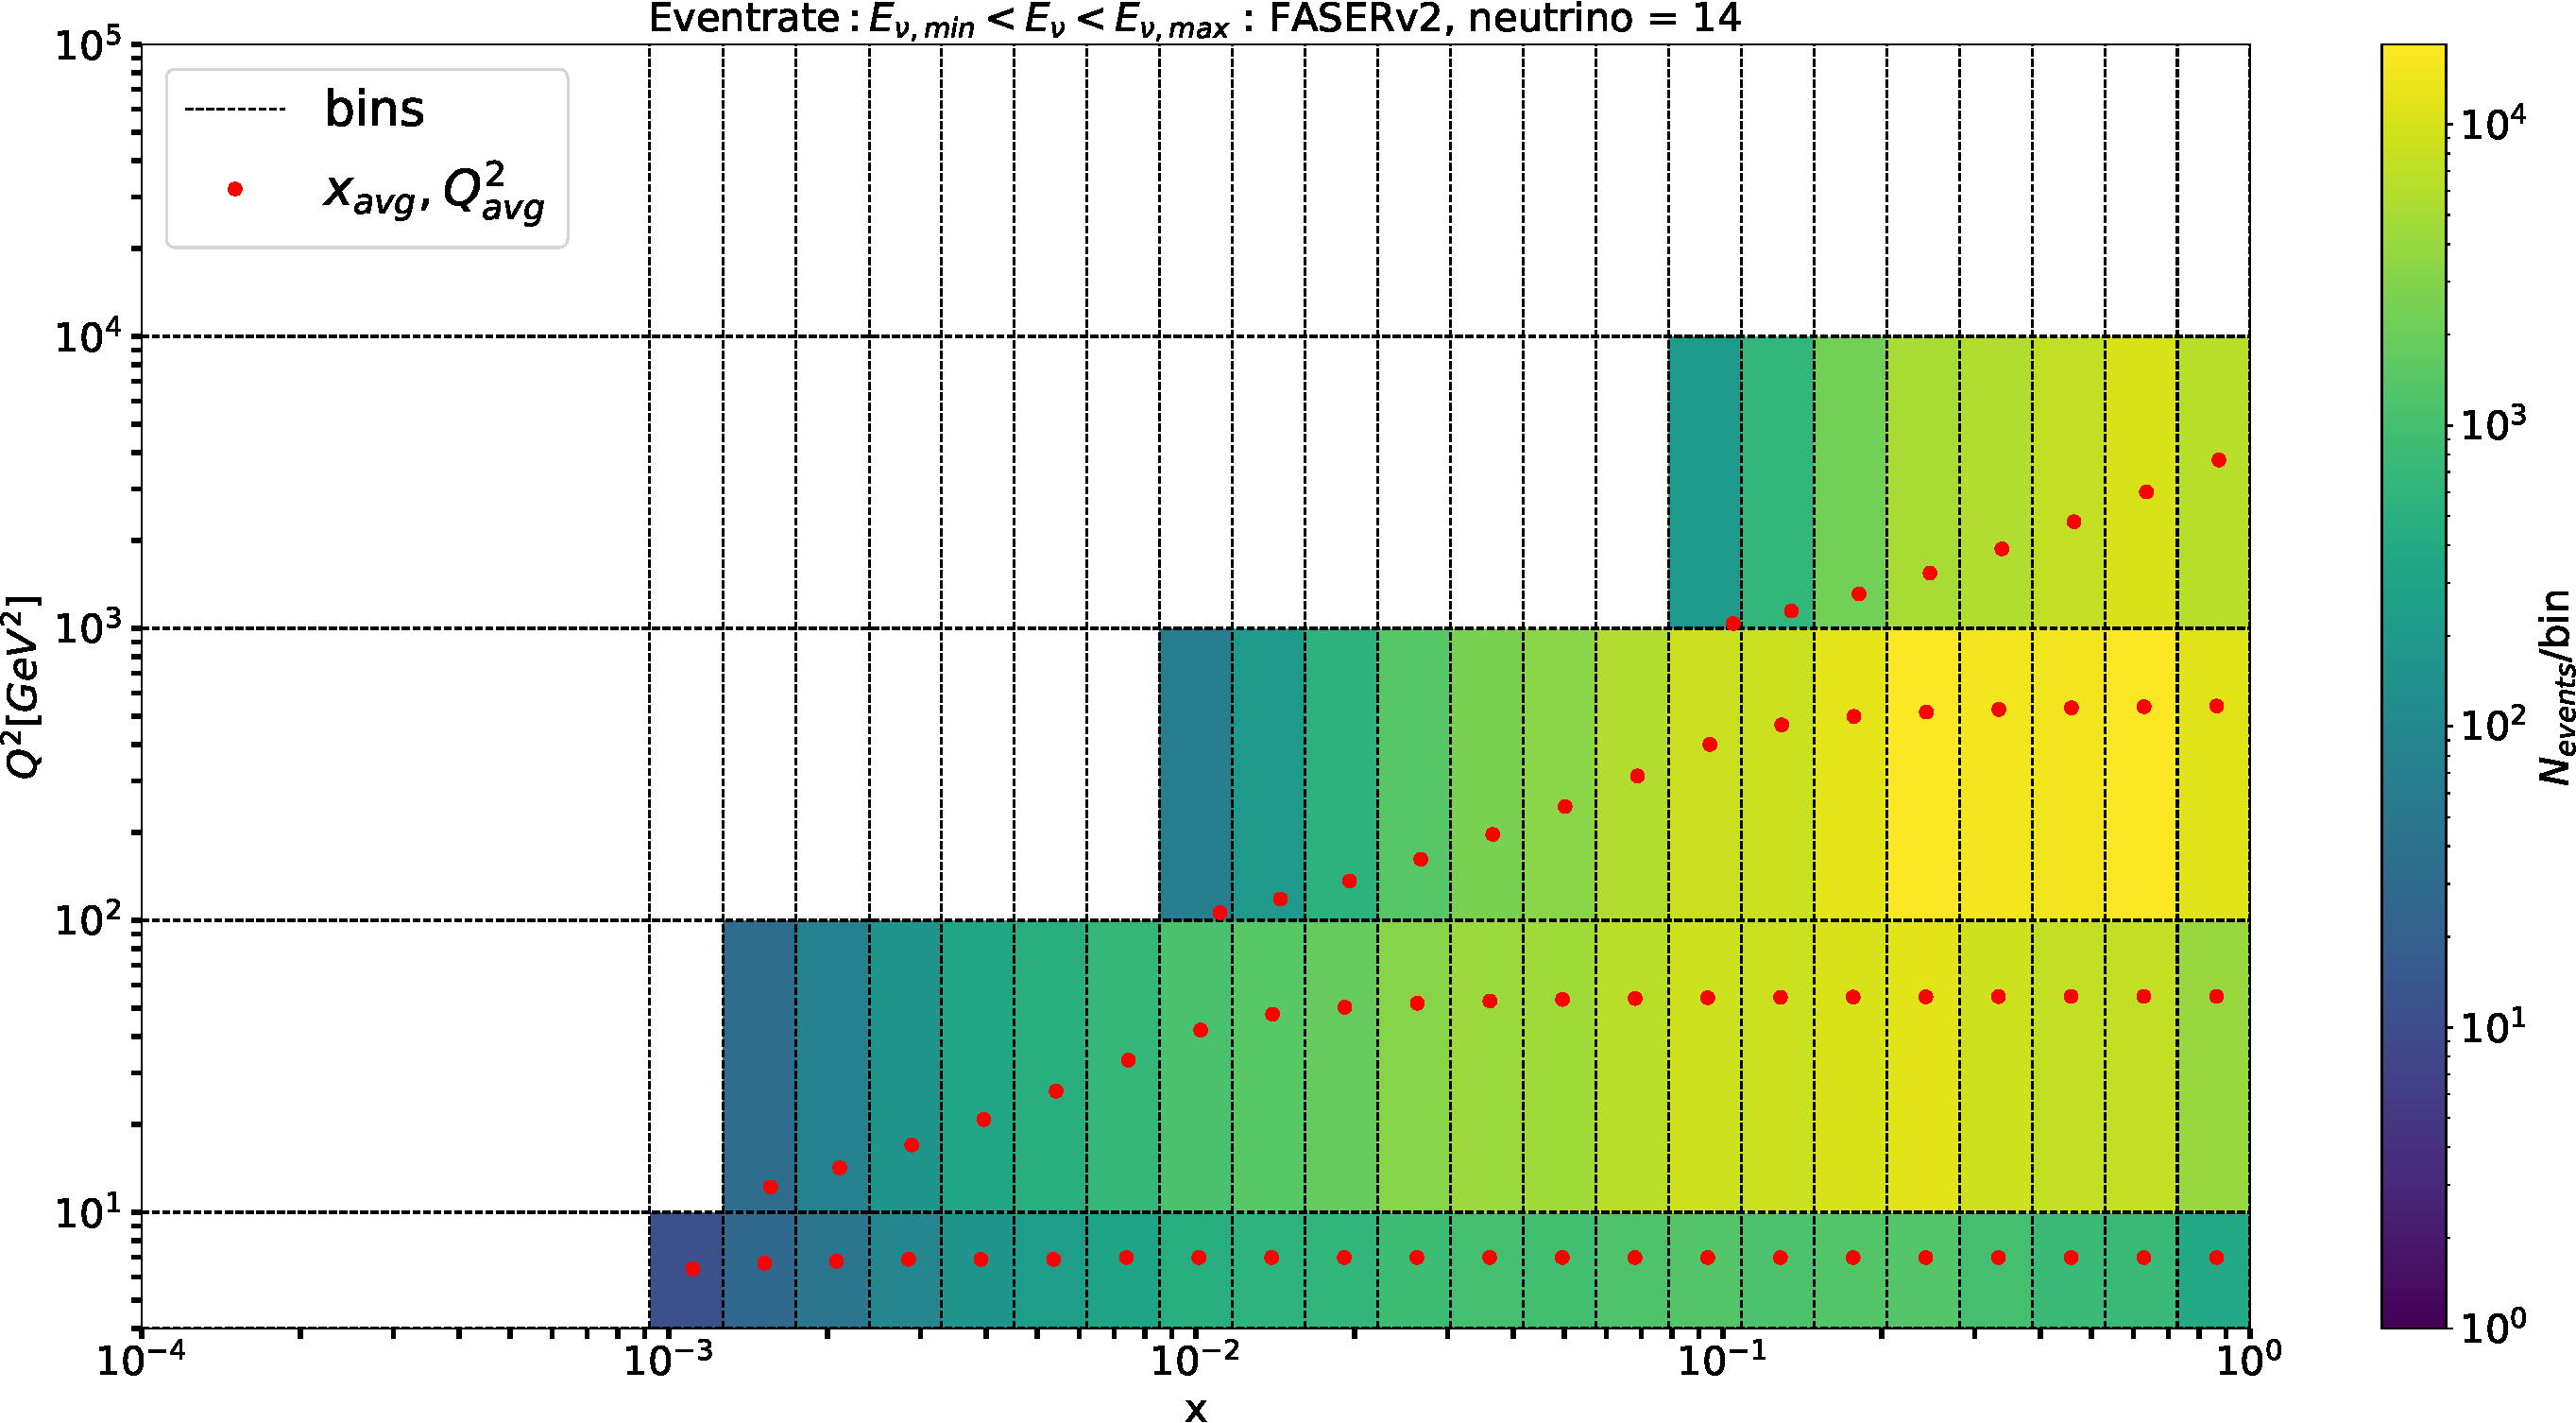
\includegraphics[width=1\textwidth]{plots/Nevent_FASERv2_14.pdf}
    \caption{Event rate per bin for muon neutrinos at FASER$\nu$2. Bins are denoted by dashed grid, and the red dot indicates the weighted average of $x,Q^2$ points in each bin. The total number of muon neutrino events calculated is $\approx2.6\times 10^5$. Note that bins were chosen somewhat arbitrarily, and can be iterated to improve PDF fits }
    \label{fig:fasernu2_muon}
\end{figure}

\subsection{Systematic Effects on Pseudodata}
We now wish to understand the impact of systematic uncertainties on the event rate in $(x,Q^2,E_{\nu})$ space. For each experiment, the observables $E_{l},E_{h},\theta$ are related to $(x,Q^2,E_{\nu})$ by 

\begin{align}
E_{\nu} = E_l + E_h \nonumber \\
Q^2 = 4E_lE_{\nu}\sin^2{\theta/2} \nonumber \\
x = \frac{Q^2}{2m_N(E_{\nu} - E_l)}.
\end{align}

We wish to sample over the space of observables, $(E_{l},E_{h},\theta)$, perform  cuts based on detector performance, calculate the event rates, and then smear this sampling according to experimental uncertainties to estimate the uncertainty on the event rate. 

Taking FASER${\nu}$2 as an example, we can write the experimental cuts and uncertainties as 

\begin{align}
100 < E_l < E_{\nu,{\rm max}} , \delta E_l = 30\% \nonumber \\
100 < E_h < E_{\nu,{\rm max}} , \delta E_h = 50\% \nonumber \\
0 < \theta < \tan^{-1}(0.5) , \delta\theta = 1~{\rm mrad}
\label{fasernu2systematic_errors}
\end{align}

We first generate a MC dataset, $D_0$, over this space with $N = 10^7$ samples and calculate $x,Q^2,E_{\nu}$ for each event, removing samples with $y > 1$. We then integrate according to Eq. \ref{MCintegration} to produce a distribution of events with bins in $x,Q^2,E_{\nu}$. We then smear each sample according to a Gaussian distribution with widths given by Eq.~\ref{fasernu2systematic_errors} to produce a new data set $D_i$ and repeat to produce $M = 10$ event distributions($M>10$ can later be used, but $M = 10$ appears to be stable). For each bin we take the standard deviation to produce the systematic errors per bin (denoted as "N\textunderscore sys\textunderscore errs" in files named "binned\textunderscore sys-events... .txt" \href{https://github.com/juanrojochacon/FPF-WG1/tree/main/results}{here}). 

For FASER${\nu}$2, the systematic errors typically dominate over statistical errors, at about $10\%$. 

\begin{figure}[h]
    \centering
    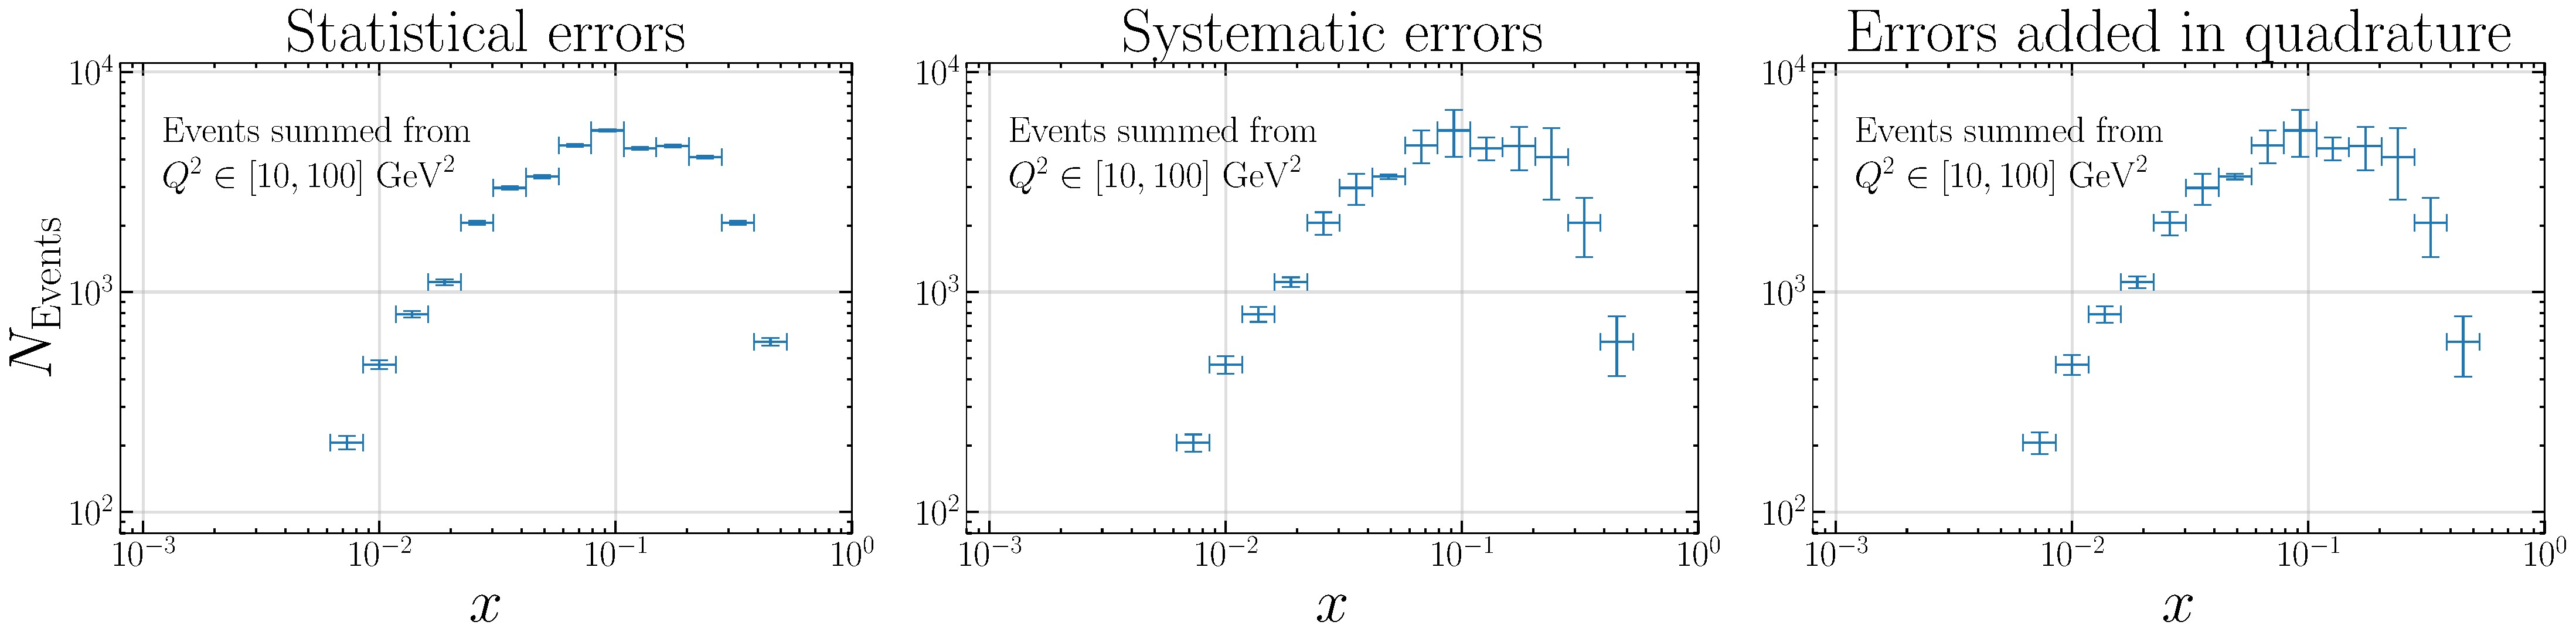
\includegraphics[width = 1\textwidth]{plots/error_plot_FASERv2_14.pdf}
    \caption{Event rates with error bars at FASER$\nu$2 for $\nu_{\mu} N \rightarrow \mu^- X$} summed over $Q^2$. The error bars along the x-axis showing the width of the $x$-bins, and are not showing any type of error.
    \label{fig:my_label}
\end{figure}

\subsection{Experimental acceptance performance} 

\paragraph{AdvSND} 
\begin{itemize}
    \item The detectors will be able to track muons that have energy greater
    than $20~\rm{GeV}$ (the values for the other charged leptons remain to be
    determined) with an acceptance angle of 100 mrad for the muons and 
    500 mrad for the both electrons and tau.
    \item In addition, the information on the charge of the outgoing leptons
    can also be accessed.
    \item It should also be possible to reconstruct the hadronic final states
    by measuring the total energy.
\end{itemize}

\paragraph{FLArE}
\begin{itemize}
    \item The detectors will be able to detect electrons with energy up to
    $1~\rm{TeV}$ and an acceptance angel as high as 0.5 rad. For the muons,
    the detectors will only be able to track them up to $1.5~\rm{GeV}$ with
    a scattering angle reaching up to 0.4 mrad. The reconstruction of the
    tau's angle and energy instead will be very difficult. However, it might
    be possible to find the vertex of a particular tau decay if fine position
    resolution is achieved.
    \item With the current baseline design of the detector, it will not be
    possible to access the information on the sign of the charged leptons.
    \item It should also be possible to reconstruct the hadronic final
    states but the reconstruction efficiency and particles will depend on
    the type of particles. It is expected that the final states hadrons will
    be dominated by pions, protons, and neutrons.
    \item Regarding the systematic errors on the charged lepton energy and
    scattering angle, it is expected to get $5\%$ energy resolution for
    electrons and about 15 mrad in angular resolution. Due to the large
    missing energy in the detector, $30\%$ energy resolution is probably
    achievable for muons with about 5 mrad angular resolution.
\end{itemize}
